% Template for Cogsci submission with R Markdown

% Stuff changed from original Markdown PLOS Template
\documentclass[10pt, letterpaper]{article}

\usepackage{cogsci}
\usepackage{pslatex}
\usepackage{float}
\usepackage{caption}

% amsmath package, useful for mathematical formulas
\usepackage{amsmath}

% amssymb package, useful for mathematical symbols
\usepackage{amssymb}

% hyperref package, useful for hyperlinks
\usepackage{hyperref}

% graphicx package, useful for including eps and pdf graphics
% include graphics with the command \includegraphics
\usepackage{graphicx}

% Sweave(-like)
\usepackage{fancyvrb}
\DefineVerbatimEnvironment{Sinput}{Verbatim}{fontshape=sl}
\DefineVerbatimEnvironment{Soutput}{Verbatim}{}
\DefineVerbatimEnvironment{Scode}{Verbatim}{fontshape=sl}
\newenvironment{Schunk}{}{}
\DefineVerbatimEnvironment{Code}{Verbatim}{}
\DefineVerbatimEnvironment{CodeInput}{Verbatim}{fontshape=sl}
\DefineVerbatimEnvironment{CodeOutput}{Verbatim}{}
\newenvironment{CodeChunk}{}{}

% cite package, to clean up citations in the main text. Do not remove.
\usepackage{apacite}

% KM added 1/4/18 to allow control of blind submission


\usepackage{color}

% Use doublespacing - comment out for single spacing
%\usepackage{setspace}
%\doublespacing


% % Text layout
% \topmargin 0.0cm
% \oddsidemargin 0.5cm
% \evensidemargin 0.5cm
% \textwidth 16cm
% \textheight 21cm

\title{Pressure to communicate across knowledge asymmetries leads to
pedagogical-like language input}


\author{{\large \bf Benjamin C. Morris} \\ \texttt{benmorris@uchicago.edu} \\ Department of Psychology \\ University of Chicago \And {\large \bf Daniel Yurovsky} \\ \texttt{yurovsky@uchicago.edu} \\ Department of Psychology \\ University of Chicago}

\begin{document}

\maketitle

\begin{abstract}
Infants prefer to listen to and learn better from child-directed speech.
This speech might support learning in part due to communicative
pressure: parents must use language that their children understand. We
present longitudinal corpus data of parent-child interaction to
demonstrate that parents provide information-rich referential
communication (using both gesture and speech during the same reference)
more for infrequent referents and when their children are younger. We
then present a Mechanical Turk study to experimentally validate this
idea, asking Turkers to communicate with a listener who a novel language
less well. Participants could communicate in 3 ways: pointing (expensive
but unambiguous), labelling (cheap but knowledge-dependent), or both.
They won points only for communicating successfully; using pointing and
labelling together was costly, but could teach, allowing cheaper
communication on later trials. Participants modulated their
communicative behavior in response to their own and their partner's
knowledge and teaching emerged when the speaker had substantially more
knowledge of the lexicon. While language is more than reference games,
this work validates the hypothesis that communicative pressure alone can
lead to supportive language input.

\textbf{Keywords:}
Language; Child-Directed Speech; POMDP.
\end{abstract}

\section{Introduction}\label{introduction}

One of the most striking aspects of children's language learning is just
how quickly they master the complex system of their natural language
(Bloom, 2000). In just a few short years, children go from complete
ignorance to conversational fluency that is the envy of second-language
learners attempting the same feat later in life (Newport, 1990). What
accounts for this remarkable transition?

One possibility is that children's caregivers deserve most of the
credit; that the language parents produce to their children is optimized
for teaching. Although there is some evidence that aspects of
child-directed speech support learning, other aspects--even in the same
subproblem, e.g.~phoneme discrimination--appear to make learning more
difficult (Eaves Jr, Feldman, Griffiths, \& Shafto, 2016; McMurray,
Kovack-Lesh, Goodwin, \& McEchron, 2013). In general, parents rarely
explicitly correct their children, and children are resistant to the
rare explicit language correction they do get (Newport, Gleitman, \&
Gleitman, 1977). Thus while parents may occasionally offer a supervisory
signal, the bulk of the evidence suggests that parental supervision is
unlikely to explain rapid early language acquisition

Alternatively, even the youngest infants may already come to language
acquisition with a precocious ability to learn the latent structure of
language from the statistical properties of speech in their ambient
environment (Saffran \& 2003, 2003; L. B. Smith \& Yu, 2008). While a
number of experiments clearly demonstrate the early availability of such
mechanisms, there is reason to be suspicious about just how precocious
they are early in development. For example, infants' ability to track
the co-occurrence information connecting words to their referents
appears to be highly constrained by both their developing memory and
attention systems (\textbf{Vlach2013}) (L. B. Smith \& Yu, 2013).
Further, computational models of these processes show that the rate of
acquisition is highly sensitive to variation in environmental statistics
(Blythe, Smith, \& Smith, 2010; Vogt, 2012). Thus precocious
unsupervised statistical learning also appears to fall short of an
explanation for rapid early language learning.

We explore the consequences of a third possibility: The language that
children hear is neither designed for pedagogy, nor is it random; it is
designed for communication (Brown, 1977). We take as the caregiver's
goal the desire to communicate with the child, not about language
itself, but instead about the world in front of them. To succeed, the
caregiver must produce the kinds of communicative signals that the child
can understand, and thus might tune the complexity of their speech not
for the sake of learning itself, but as a byproduct of in-the-moment
pressure to communicate successfully (Yurovsky, 2017).

To examine this hypothesis, we first analyze parent communicative
behavior in a longitudinal corpus of parent-child interaction in the
home (\textbf{Goldin-Meadow et al., 2014}). We investigate the extent to
which parents modify their communicative behavior across their child's
development to align to their child's developing linguistic knowledge.
\textbf{?maybe something about alignment at other levels, syntatic,
lexical, etc.,--\textgreater{} but we're looking here for modality?}
Specifically, we analyze communicative modality to look for instances
gesture-speech co-occurence-- when speakers indicate the same referent
in two modalities. These instances might be particularly powerful
learning opportunities for young children because they provide a verbal
label in the presence of a highly disambuiguting gestural cue (e.g.,
pointing, holding), greatly reducing referential uncertainty
(\textbf{gesture-speech citation, word-learning as uncertainty
reduction}).

\subsection{even for words they know}\label{even-for-words-they-know}

We then turn to the emergence of alignment in a simple model system: an
iterated reference game in which two players earn points for
communicating successfully with each other. On each round of the game,
participants can point--a signal which is costly to produce but always
communicatively effective, or can use language--a cheaper signal which
is cheap to produce but successful only if both players share a common
lexicon. Crucially, participants can point and speak together--paying
the cost of both, but effectively establishing a shared label for this
referent that they can exploit on later trials of the game.

In an experiment on Mechanical Turk using this model system, we show
that people tune their communicative to choices to varying cost and
reward structures, and also critically to their partner's linguistic
knowledge--teaching when partners are unlikely to know language and many
more rounds remain. We then show that human behavior can be explained by
a rational planning model that seeks to optimize its total expected
utility over the course of the game. Together, these data show that
pedagogically-supportive input can arise from purely selfish motives to
maximize the utility of communicating successfully while minimizing the
cost of communication. We take these results as a proof of concept that
both the features of child-directed speech that support learning as well
as those that inhibit it may arise from a single unifying goal: The
desire to communicative efficiently.

\section{Corpus Data}\label{corpus-data}

To begin with, we investigate aligned linguisitc input in naturalistic,
parent-child corpus data. We focus on parent referential communication
to examine how might be aligning to their children. The degree of
parental alignment should be sensitive to the child's age, such that
parents will be more likely to provide richer communicative information
when their child is younger, when she has less linguistic knowedge, than
as she gets older (Yurovsky, Doyle, and Frank, 2016). Parental alignment
should also be stronger for infrequent objects, where again children are
likely to have less knowledge of the relevant label. We analyze the
production of gesture-speech cooccurence for the same referent, in the
same instance, which could reflect alignment if parents are senstively
using this information-rich cue for young children and infrequent
objects.

\subsubsection{Participants, Materials,
Methods}\label{participants-materials-methods}

These data come from the Language Development Project, a large-scale,
longitudinal corpus of parent child-interaction in the home with
families whose socio-economic, racial, and gender diversity is
representative of the broader Chicago community (Goldin-Meadow et al.,
2014)\ldots{} \textbf{add specific demographics info}

These data are drawn from a sample of 10 families from the greater
corpus. Recordings were taken in the home every 4-months from when the
child was 14-months-old until they were 34-months-old, resulting in 6
timepoints (missing one family at the 30-month timepoint). Recordings
were 90 minute sessions, and participants were given no instructions.

\paragraph{Corpus Coding}\label{corpus-coding}

The Language Development Project corpus contains transcription of all
speech and communicative gestures prroeduced by children and their
caregivers over the course of the 90-minute home recordings. An
indpendent coder analyzed each of these communicative instances and
identified each time a concrete noun was referenced using speech (i.e.,
a specific noun form) or gesture (only deictic gestures were coded for
ease of coding and interpretation).

\textbf{ask maddie about criteria for `both' coding, couldn't find in
the manual}

\begin{CodeChunk}
\begin{figure*}[h]

{\centering 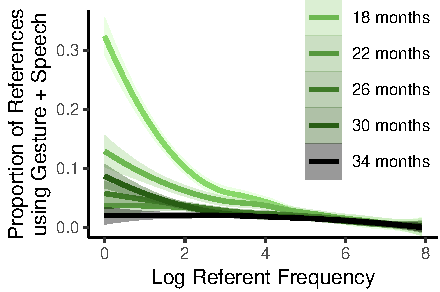
\includegraphics{figs/corpus_plot-1} 

}

\caption[Proportion of parent referential talk with speech-gesture cooccurence across development]{Proportion of parent referential talk with speech-gesture cooccurence across development. Lines represent child's age (14-34 months). The log of the referent's frequency is given on the x-axis, where more infrequent items are closer to zero.}\label{fig:corpus_plot}
\end{figure*}
\end{CodeChunk}

\subsubsection{Results}\label{results}

These corpus data were analyzed using a mixed effects regression to
predict parent use of gesture-speech cooccurence for a given referent.
Random effects of subject and referent were included in the model. Our
key predictors were child age and referent frequency * is this spoken
frequency in the corpus overall? *.

We find a signficant negative effect of age, such that parents are
signficantly less likely to provide the gesture-speech cue as their
child gets older (\emph{B} \textless{} -0.038, \emph{p \textless{}
0.0001}).

\section{Experimental Framework}\label{experimental-framework}

To study the emergence of pedagogy from communicative pressure, we
developed a simple reference game in which participants would be
motivated to communicate successfully. After giving people varying
amounts of training on novel names for 6 novel objects, we asked them to
play a communicative game in which they were given one of the objects as
their referential goal, and they were rewarded if their partner
successfully selected this referent from among the set of competitors
(Figure \ref{fig:imp_screenshot}). Participants could choose to refer
either using the novel labels they had been exposed to, or they could
use a deictic gesture to indicate the referent to their partner. Deixis
was unambiguous, and thus would always succeed. However, in order for
language to be effective, the participant and their partner would have
to know the correct novel label for the referent. Across participants,
we varied the relative cost of using these two communicative signals.

If people are motivated to communicate successfully, their choice of
referential modality should reflect the tradeoff between the cost of
producing the communicative signal with the likelihood that the
communication would succeed. We thus predicted that peoples' choice of
referential modality would reflect this calculus: People should be more
likely to use language if they have had more exposures to the novel
object's correct label, and they should be more likely to use language
as gesture becomes relatively more costly.

Across 12 conditions, 480 participants were recruited to play our
reference game via Amazon Mechanical Turk, an online platform that
allows workers to complete surveys and short tasks for payment. In this
study, all participants were placed in the role of speaker and listener
responses were programmed.

\begin{CodeChunk}
\begin{figure}[H]

{\centering 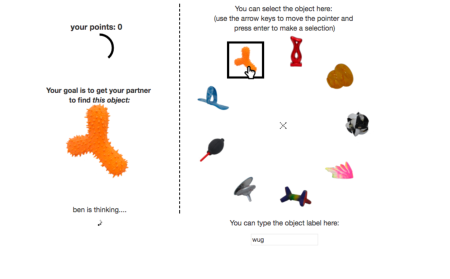
\includegraphics{figs/imp_screenshot-1} 

}

\caption[Screenshot of speaker view during gameplay]{Screenshot of speaker view during gameplay.}\label{fig:imp_screenshot}
\end{figure}
\end{CodeChunk}

\section{Amazon Turk Experiment}\label{amazon-turk-experiment}

In this experiment, we explicitly implemented strategy utility by
assigning point values to each communicative method. Experiment 1
provides a proof of concept to show that participants were sensitive to
our manipulation and that we could induce speech-gesture tradeoff with
this paradigm.

\subsubsection{Participants, Materials,
Methods}\label{participants-materials-methods-1}

480 participants were recruited though Amazon Mechanical Turk and
received a small payment for their participation. Data from \textbf{XYZ}
participants was excluded from subsequent analysis for failing the
manipulation check or for producing pseudo-English labels (e.g.,
`pricklyyone').

Participants were told they would be introduced to novel object-label
pairs and then asked to play a communication game with a partner wherein
they would have to refer to a particular target object. Participants
were exposed to nine novel objects, each with a randomly assigned
pseudo-word label. We manipulated the degree of exposure within
subjects, such that, during training, participants saw two of the six
object-label mappings five times, three times, or two time, resulting in
a total of 20 training trials. Participants were then given a simple
recall task to establish their baseline knowledge of the novel lexicon
(pretest).

After being introduced to the rules of the game, participants are
screened to ensure they understand key aspects of the manipulation,
i.e.~their partner's knowledge and the number of times each object would
be discussed during subsequent gameplay (manipulation check). During
gameplay, speakers saw the target object in addition to an array of all
six objects (see Figure \ref{fig:imp_screenshot} for the speaker's
perspective). Speakers had the option of either directly selecting the
target object from the array (gesture)- a higher cost cue but without
ambiguity- or typing a label for the object (speech)- a lower cost cue
but contingent on the listener's knowledge. After sending the message,
speakers are shown which object the listener selected.

Additionally, particpants were told about a third type of message using
both gesture and speech within a single trial to effectively teach the
listener an object-label mapping. In order to produce this teaching
behavior, speakers had to pay the cost of producing both cues (i.e.~the
time it takes to type the label and select the referent using the arrow
keys). Our communicative game was designed to reward in-the-moment
communication, and thus teaching required the speaker paying a higher
cost upfront. However, rational communicators may understand that if one
is accounting for future trials, paying the cost upfront to teach the
listener allows a speaker to use a less costly message strategy on
subsequent trials (namely, speech).

Incorporating teaching means that our speaker must now reason about
their interlocutor's knowledge state more explicitly, in order to make
rational decisions about what to teach and when. To address this added
dimension, we also manipulated participants' expectations about their
partner's knowledge. Prior to beginning the game, participants were told
that there partner had either no experience with the lexicon, had half
the experience of the speaker, the same experience, or had twice the
experience of the speaker.

Listeners starting knowledge state were also initialized accordingly.
Listeners with no exposure were given no knowledge of the lexicon to
start. Listeners with half the exposure of the speaker began with
knowledge of three object-label pairs (2 high frequency, 1 mid
frequency), based the average retention rates found previously.
Listeners with the same exposure of the speaker began with knowledge of
three object-label pairs (2 high frequency, 2 mid frequency, 1 low
frequency), again based the average retention rates found previously.
Lastly, the listener with twice as much exposure as the speaker began
with perfect knowledge of the lexicon. Through gesture-speech
co-occurrence, the speaker could effectively teach the listener a novel
mapping. \ldots{} Listeners could learn a novel mapping from one
teaching event in this game and integrate it into their set of candidate
words when evaluating the LD of subsequent labels\ldots{}

Speakers could win up to 100 points per trial if the listener correctly
selected the target referent based on their message. If the listener
failed to identify the target object, the speaker received no points. We
manipulated the relative utilities of each of the strategies
between-subjects, emb the relative utilities of the communicative
strategies in the gameplay more implicitly. Using a timer that
controlled the number of points that were earned on each trial of
gameplay (Figure \ref{fig:imp_screenshot}). Rather than impose an
explicit point system, we set the relative utilities of communication
strategies by manipulating the speed with which participants could
respond.

During the game, the six novel objects were arranged in a circle around
a cartoon pointer (see Figure \ref{fig:imp_screenshot}). To manipulate
the relative speeds of gesturing and labeling, we required speakers to
move a small pointer using the arrow keys on their keyboards in order to
select an object with gesture. With this method we could directly
manipulate the speed of the pointer while holding the arrow keys to
effectively set the maximum possible utility of using gesture.

If the listener correctly identified the target object, speakers
received points determined by the amount of time remaining on the timer.
For successful communications, speakers always received a minimum of 10
points, regardless of the time elapsed. Based on pilot response times,
the timer was set to 6.5 seconds. The timer did not begin until speakers
began an action (i.e.~pressed a key), so that speed of recall would not
be an additional cost. Participants were randomly assigned into one of
three conditions, where the pointer was set to either a fast, slow, or
slowest setting. \textbf{more on how speed works// quantitative?}

This framework allowed us to implement the point system as an implicit
extension of gameplay and resulted in each participant having unique
gesture-speech utilities, based on the speed of their responses across
the two methods. \textbf{Plot the average points for a given speed
condition?, or put a table in?}

\subsubsection{Results}\label{results-1}

As expected, participants were sensitive to both the exposure rate and
the relative utilities of the communication strategies. As an initial
check of our knowledge manipulation, a logistic regression indicated
that the more exposures to a given object-label pair during training,
the more likely participants were to recall that label at pretest (B =
XYZ, p \textless{} XYZ).

\paragraph{Gesture-Speech Tradeoff}\label{gesture-speech-tradeoff}

A separate logistic regression was used to predict whether speakers
chose to produce a gesture or a label during a given trial as a function
of the exposure rate and utility manipulation. There was a significant
effect of exposure rate such that the more exposures to a particular
object-label pair during training, the more likely a speaker was to
produce a label (B = 0.48, p \textless{} 0.001). Participants also
modulated their communicative behavior on the basis of the utility
manipulation. Speakers in the Talk is Cheap condition produced
significantly more labels than participants in the Talk is Less Cheap
condition (B = 0.61, p \textless{} 0.001). Thus, participants are
sensitive to our manipulations- altering their choices about how to
communicate with their partner on the basis of their own knowledge, the
degree of training, and the imposed utilities.

In Experiment 3, we see gesture and speech trading off in the same
patterns as Experiments 1 and 2. A mixed effects logistic regression
showed that the more exposure to a given object during training, the
more likely speakers were to label that object during the game (B =
0.53, p \textless{} 0.01)\ldots{}.

\ldots{}.. Critically, there was a main effect of our utility
manipulation, such that speakers the more difficult it was to gesture,
the more likely participants were to rely on speech (B = 0.09, p
\textless{} 0.01). Figure \ref{fig:imp_speech_gesture} illustrates this
pattern in the condition where the listener has more exposure than the
speaker, as there was minimal teaching in that condition and thus the
speech-gesture trade-off is most interpretable. In the absence of an
explicit framework for assigning utilities based on method, speakers
continue to adapt their communicative choices taking into account the
expected utility of possible strategies.

\begin{CodeChunk}
\begin{figure}[H]

{\centering 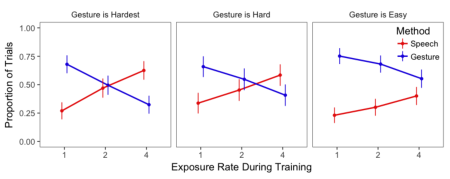
\includegraphics{figs/imp_speech_gesture-1} 

}

\caption[Speakers' communicative method choice as a function of exposure and the utility manipulation]{Speakers' communicative method choice as a function of exposure and the utility manipulation. These data are taken only from the condition where listeners had more exposure to the lexicon than speakers, as the speech-gesture trade-off is most easily interpreted here. Rates of teaching not show.}\label{fig:imp_speech_gesture}
\end{figure}
\end{CodeChunk}

\paragraph{Emergence of Teaching}\label{emergence-of-teaching}

Thus far, we have focused on relatively straightforward scenarios to
demonstrate that a pressure to communicate successfully in the moment
can lead speakers to trade-off between gesture and speech sensibly.

\ldots{} In line with our hypotheses, Experiment 2 mirrored the effects
found in Experiment 1 and demonstrated that teaching is also sensitive
to these same factors. A mixed effects logistic regression predicting
whether or not teaching occurred on a given trial revealed that teaching
rates across conditions depend on all of the same factors that predict
speech and gesture. There was a significant effect of initial exposure
to the mapping on the rates of teaching, such that more exposures to a
word predicted higher rates of teaching behavior (B = 0.09, p
\textless{} 0.05). There was also a significant effect of the utility
manipulation such that being in the Talk is Cheap condition predicted
higher rates of teaching than being in the Talk is Less Cheap condition
(B = 1.07, p = 0.01), a rational response considering teaching allows
one to use a less costly strategy in the future and that strategy is
especially superior in the Talk is Cheap condition.

As a predictor in our model, we also included whether this was an
objects first, second, or third appearance in the game. The expected
utility of teaching on a given trial should decrease as there are fewer
subsequent trials for that object, thus we predicted that teaching rates
would drop dramatically. Indeed, this is consistent with the results
from our model; compared with the first appearance of an object,
speakers were significantly less likely to teach on the subsequent
appearances (B = -1.02, p \textless{} 0.001).

Nevertheless, these results corroborate our early findings,
demonstrating that teaching behavior emerges in both a paradigm with an
explicit points system (Experiment 2) and an implicit points system
(Experiment 3), despite the initial cost.

\begin{CodeChunk}
\begin{figure}[H]

{\centering 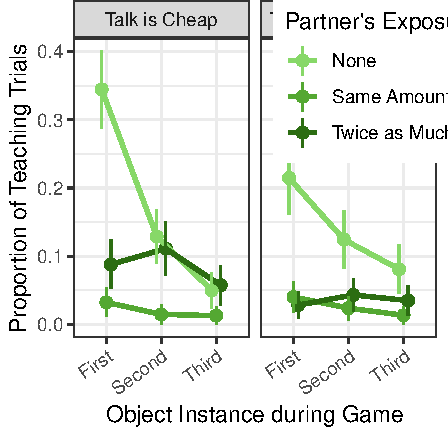
\includegraphics{figs/imp_teach-1} 

}

\caption[Rates of teaching across the partner exposure manipulation and appearances taken from gameplay in Experiment 3]{Rates of teaching across the partner exposure manipulation and appearances taken from gameplay in Experiment 3.}\label{fig:imp_teach}
\end{figure}
\end{CodeChunk}

\section{Model: Iterated Communication as Rational
Planning}\label{model-iterated-communication-as-rational-planning}

The results from this experiment are qualitatively consistent with a
model in which participants make their communicative choices to maximize
their expected utility from the reference game. We next formalize this
model to determine if these results are predicted quantitatively as
well.

\newcommand{\E}[1]{\mathbb{E}\left[ #1 \right]}

In a one-shot reference game maximizing expected utility is simply
choosing the action (\(a\)) that has the highest expected utility
\((\E{U})\). The expected utility depends both on the action itself, and
on the state of the two partners (\(s\)): For pointing, this expected
utility is independent of referent, defined entirely by our experimental
manipulation. In contrast, for speech, the utility varies with the
probability of partners sharing a common label for the referent.
Following other models in the Rational Speech Act framework, we use the
Luce Choice Axiom, in which each choice is taken in probability
proportional to its exponentiated utility (Frank \& Goodman, 2012). This
choice rule has a single parameter \(\alpha\) that controls the noise in
this choice--as \(\alpha\) approaches 0, choice is random and as
\(\alpha\) approaches infinity choice is optimal:

\[ 
C\left(a;s\right) \propto e^{\alpha \E{U \left(s,a\right))}}
\]

To use this rule, agents have to estimate how likely they are to share a
common label (\(s\)). In our simulation, we assume for simplicity that
people have an accurate representation of their own knowledge. We thus
set each simulated participant's knowledge to the explicit recall
judgment made by a real participant in our experiments. To estimate
their partner's knowledge, participants can reason about their own
learning. Again for simplicity we model learning as a simple Bernoulli
process: Each exposure to novel label is like a flipping a coin with
weight \(p\), if it comes up heads, the label is learned. Having
observed their own learning outcomes, agents can infer their own
learning rate by determining the weight \(p'\) under which their
observed learning is most likely. Assuming that their partner would have
learned at the same rate, participants can then generate a probability
with which their partner would have learned each label by estimating the
probability that at least one of its \(n\) came up heads given learning
rate \(p'\): \(P\left(s^{+}\right)=1-p'\left( 1-p' \right)^{n}\).

In an iterated game, however, because actions taken on the current trial
can influence the state (\(s\)) on future trials, the optimal action to
take is not the one that optimizes the single trial's rewards, but
rather the one that optimizes the expected rewards that will accumulate
over all future trials (Kaelbling, Littman, \& Cassandra, 1998).

For the results reported here, we set \(\alpha = 2\) based on
hand-tuning, but other values produce similar results. \textbf{also the
discounting parameter}

We implemented a two-agent model of speaker and listener behavior in
this game based on partially observable Markov decision processes. The
speaker is given a target referent each trial and must signal to the
listener which object to select. Speakers send messages to the listener
by speaking, a low cost cue that relies on the listener's knowledge, or
by pointing, a higher cost cue that is unambiguous.

The speaker estimates the listener's knowledge. First, the speaker uses
Markov chain Monte Carlo to infer their own learning rate based on how
well they were able to learn a novel lexicon after N exposures. Then,
given the listener's degree of exposure, the speaker can use their own
learning rate to infer the probability that the listener would know any
given object-label mapping. Across trials, the speaker gains further
information about the listener through their selections, allowing them
to update their beliefs about the listener's knowledge state.

The model specifies the relative costs for each communicative modality.
On each trial, the speaker estimates the expected utility of each
modality by accounting for these costs, their own knowledge of the
object's label, and the probability that the listener knows the object's
label. The speaker then uses Luce's choice axiom to select a
communicative modality based on the expected utilities.

When estimating expected utility, the model sums the expected utility of
a given trial and any remaining trials for that particular object. This
allows the speaker to engage in planning by accounting for the way a
given message may induce knowledge changes and thus affect subsequent
expected utilities. Utilities were scaled using an exponential
discounter as a function of delay to give greater weight to immediate
rewards than subsequent rewards.

Crucially, speakers can also combine both communication cues, paying the
upfront cost of both, to produce a message that is both unambiguous and
informative. In this way, speakers are able to teach their partners
object-label mappings. A speaker that plans may thus infer that teaching
the listener, especially if there is an asymmetry in their knowledge
states, may have a high expected utility after accounting for remaining
trials where the speaker could use a less costly cue (i.e.~speech).
After producing both cues, the speaker also updates their own beliefs
about the partner's knowledge state to reflect this exposure.

\begin{CodeChunk}
\begin{figure}[H]

{\centering 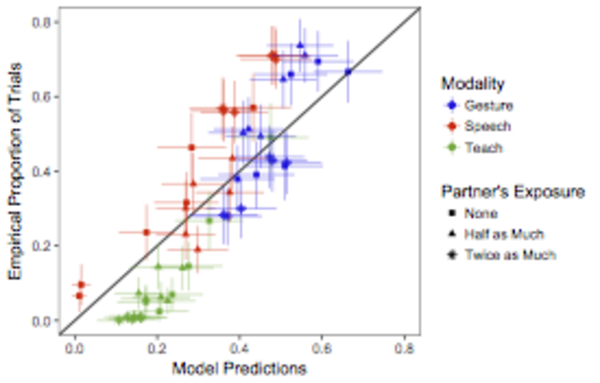
\includegraphics{figs/image4-1} 

}

\caption[Plot of the fit between model predictions and empirical data]{Plot of the fit between model predictions and empirical data.}\label{fig:image4}
\end{figure}
\end{CodeChunk}

\section{General Discussion}\label{general-discussion}

is it worth having preliminary discussions at the end of the corpus
section, and the experiment section?

limitations- obviously different pressures on the model feedback (fewer
interactions, half situation don't know knowledge, no in-the-moment
pressures like drift model\ldots{} gesture when speech is slow to
come\ldots{}).

this idea isn't specific to gesture-speech coocurrence.

\section{Acknowledgements}\label{acknowledgements}

We are grateful to Elliot Lipnowski for thoughtful feedback on the
model, to Susan Goldin-Meadow for sharing access to the Language
Devleopment Project data, and to Madeline Meyers for help in coding and
analyzing the corpus data. This research was funded by a James S.
McDonnell Foundation Scholar Award to DY.

\hypertarget{refs}{}
\hypertarget{ref-bloom2000}{}
Bloom, P. (2000). \emph{How children learn the meanings of words}. MIT
press: Cambridge, MA.

\hypertarget{ref-blythe2010}{}
Blythe, R. A., Smith, K., \& Smith, A. D. M. (2010). Learning times for
large lexicons through cross-situational learning. \emph{Cognitive
Science}, \emph{34}, 620--642.

\hypertarget{ref-brown1977}{}
Brown, R. (1977). Introduction. In C. E. Snow \& C. A. Ferguson (Eds.),
\emph{Talking to children: Language input and interaction}. Cambridge,
MA.: MIT Press.

\hypertarget{ref-eaves-jr2016}{}
Eaves Jr, B. S., Feldman, N. H., Griffiths, T. L., \& Shafto, P. (2016).
Infant-directed speech is consistent with teaching. \emph{Psychological
Review}, \emph{123}(6), 758.

\hypertarget{ref-frank2012}{}
Frank, M. C., \& Goodman, N. D. (2012). Predicting Pragmatic Reasoning
in Language Games. \emph{Science}, \emph{336}(6084), 998--998.

\hypertarget{ref-kaelbling1998}{}
Kaelbling, L. P., Littman, M. L., \& Cassandra, A. R. (1998). Planning
and acting in partially observable stochastic domains. \emph{Artificial
Intelligence}, \emph{101}, 99--134.

\hypertarget{ref-mcmurray2013}{}
McMurray, B., Kovack-Lesh, K. A., Goodwin, D., \& McEchron, W. (2013).
Infant directed speech and the development of speech perception:
Enhancing development or an unintended consequence? \emph{Cognition},
\emph{129}(2), 362--378.

\hypertarget{ref-newport1990}{}
Newport, E. L. (1990). Maturational Constraints on Language Learning.
\emph{Cognitive Science}, \emph{14}(1), 11--28.

\hypertarget{ref-newport1977}{}
Newport, E. L., Gleitman, H., \& Gleitman, L. R. (1977). Mother, I'd
rather do it myself: Some effects and non-effects of maternal speech
style. In C. A. Ferguson (Ed.), \emph{Talking to children language input
and interaction} (pp. 109--149). Cambridge University Press.

\hypertarget{ref-saffran2003}{}
Saffran, J. R., \& 2003. (2003). Statistical language learning:
Mechanisms and constraints. \emph{Current Directions in Psychological
Science}, \emph{12}(4), 110--114.

\hypertarget{ref-smith2008}{}
Smith, L. B., \& Yu, C. (2008). Infants rapidly learn word-referent
mappings via cross-situational statistics. \emph{Cognition}, \emph{106},
1558--1568.

\hypertarget{ref-smith2013}{}
Smith, L. B., \& Yu, C. (2013). Visual attention is not enough:
Individual differences in statistical word-referent learning in infants.
\emph{Language Learning and \ldots{}}, \emph{9}, 25--49.

\hypertarget{ref-vogt2012}{}
Vogt, P. (2012). Exploring the robustness of cross-situational learning
under zipfian distributions. \emph{Cognitive Science}, \emph{36}(4),
726--739.

\hypertarget{ref-yurovsky2017}{}
Yurovsky, D. (2017). A communicative approach to early word learning.
\emph{New Ideas in Psychology}, 1--7.

\bibliographystyle{apacite}


\end{document}
